% Title: Block diagram of Third order noise shaper in Compact Disc Players
% Author: Ramón Jaramillo
\documentclass{article}

\usepackage{tikz}

%\usepackage{textcomp}
\begin{document}

\begin{figure}[t]
\centering
\input{"Beacon Aggregation-BOXplot.tex"}
\hfill
\input{"Beacon Decision-BOXplot.tex"}
\hfill
\input{"Beacon Stop-BOXplot.tex"}
\caption{
Thick gray boxes represent the results of robot experiments;
Thick white boxes those of pseudo-reality; thin gray ones,
those of simulations.}
\end{figure}

\begin{figure}[t]
\centering
% Created by tikzDevice version 0.12 on 2019-03-27 16:18:26
% !TEX encoding = UTF-8 Unicode
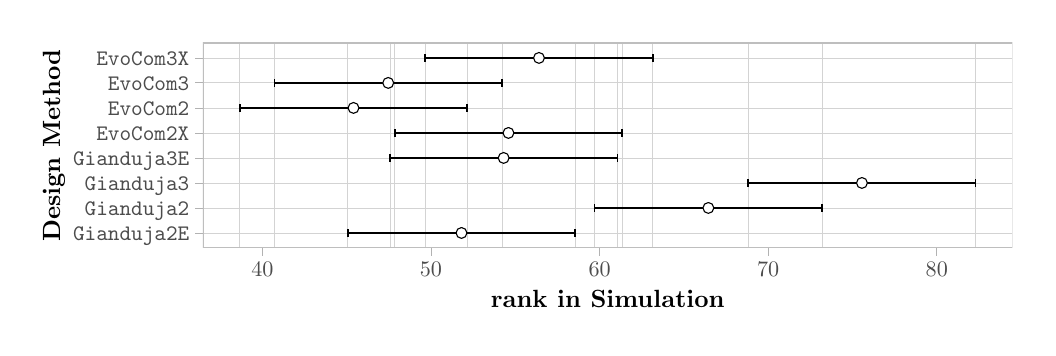
\begin{tikzpicture}[x=1pt,y=1pt]
\definecolor{fillColor}{RGB}{255,255,255}
\path[use as bounding box,fill=fillColor,fill opacity=0.00] (0,0) rectangle (361.35,108.41);
\begin{scope}
\path[clip] (  0.00,  0.00) rectangle (361.35,108.40);
\definecolor{drawColor}{RGB}{255,255,255}
\definecolor{fillColor}{RGB}{255,255,255}

\path[draw=drawColor,line width= 0.6pt,line join=round,line cap=round,fill=fillColor] (  0.00,  0.00) rectangle (361.35,108.40);
\end{scope}
\begin{scope}
\path[clip] ( 63.34, 28.81) rectangle (355.85,102.90);
\definecolor{fillColor}{RGB}{255,255,255}

\path[fill=fillColor] ( 63.34, 28.81) rectangle (355.85,102.90);
\definecolor{drawColor}{RGB}{211,211,211}

\path[draw=drawColor,line width= 0.3pt,line join=round] ( 63.34, 79.41) --
	(355.85, 79.41);

\path[draw=drawColor,line width= 0.3pt,line join=round] ( 63.34, 88.45) --
	(355.85, 88.45);

\path[draw=drawColor,line width= 0.3pt,line join=round] ( 63.34, 43.27) --
	(355.85, 43.27);

\path[draw=drawColor,line width= 0.3pt,line join=round] ( 63.34, 34.23) --
	(355.85, 34.23);

\path[draw=drawColor,line width= 0.3pt,line join=round] ( 63.34, 52.30) --
	(355.85, 52.30);

\path[draw=drawColor,line width= 0.3pt,line join=round] ( 63.34, 61.34) --
	(355.85, 61.34);

\path[draw=drawColor,line width= 0.3pt,line join=round] ( 63.34, 97.48) --
	(355.85, 97.48);

\path[draw=drawColor,line width= 0.3pt,line join=round] ( 63.34, 70.37) --
	(355.85, 70.37);

\path[draw=drawColor,line width= 0.2pt,line join=round] (158.83, 28.81) -- (158.83,102.90);

\path[draw=drawColor,line width= 0.2pt,line join=round] (214.83, 28.81) -- (214.83,102.90);

\path[draw=drawColor,line width= 0.2pt,line join=round] (171.38, 28.81) -- (171.38,102.90);

\path[draw=drawColor,line width= 0.2pt,line join=round] (225.85, 28.81) -- (225.85,102.90);

\path[draw=drawColor,line width= 0.2pt,line join=round] (287.07, 28.81) -- (287.07,102.90);

\path[draw=drawColor,line width= 0.2pt,line join=round] (197.85, 28.81) -- (197.85,102.90);

\path[draw=drawColor,line width= 0.2pt,line join=round] (342.55, 28.81) -- (342.55,102.90);

\path[draw=drawColor,line width= 0.2pt,line join=round] (213.08, 28.81) -- (213.08,102.90);

\path[draw=drawColor,line width= 0.2pt,line join=round] ( 76.64, 28.81) -- ( 76.64,102.90);

\path[draw=drawColor,line width= 0.2pt,line join=round] (132.64, 28.81) -- (132.64,102.90);

\path[draw=drawColor,line width= 0.2pt,line join=round] ( 89.19, 28.81) -- ( 89.19,102.90);

\path[draw=drawColor,line width= 0.2pt,line join=round] (143.66, 28.81) -- (143.66,102.90);

\path[draw=drawColor,line width= 0.2pt,line join=round] (204.88, 28.81) -- (204.88,102.90);

\path[draw=drawColor,line width= 0.2pt,line join=round] (115.66, 28.81) -- (115.66,102.90);

\path[draw=drawColor,line width= 0.2pt,line join=round] (260.36, 28.81) -- (260.36,102.90);

\path[draw=drawColor,line width= 0.2pt,line join=round] (130.89, 28.81) -- (130.89,102.90);
\definecolor{drawColor}{RGB}{0,0,0}

\path[draw=drawColor,line width= 0.6pt,line join=round] (158.83, 78.06) --
	(158.83, 80.77);

\path[draw=drawColor,line width= 0.6pt,line join=round] (158.83, 79.41) --
	( 76.64, 79.41);

\path[draw=drawColor,line width= 0.6pt,line join=round] ( 76.64, 78.06) --
	( 76.64, 80.77);

\path[draw=drawColor,line width= 0.6pt,line join=round] (214.83, 69.02) --
	(214.83, 71.73);

\path[draw=drawColor,line width= 0.6pt,line join=round] (214.83, 70.37) --
	(132.64, 70.37);

\path[draw=drawColor,line width= 0.6pt,line join=round] (132.64, 69.02) --
	(132.64, 71.73);

\path[draw=drawColor,line width= 0.6pt,line join=round] (171.38, 87.09) --
	(171.38, 89.80);

\path[draw=drawColor,line width= 0.6pt,line join=round] (171.38, 88.45) --
	( 89.19, 88.45);

\path[draw=drawColor,line width= 0.6pt,line join=round] ( 89.19, 87.09) --
	( 89.19, 89.80);

\path[draw=drawColor,line width= 0.6pt,line join=round] (225.85, 96.13) --
	(225.85, 98.84);

\path[draw=drawColor,line width= 0.6pt,line join=round] (225.85, 97.48) --
	(143.66, 97.48);

\path[draw=drawColor,line width= 0.6pt,line join=round] (143.66, 96.13) --
	(143.66, 98.84);

\path[draw=drawColor,line width= 0.6pt,line join=round] (287.07, 41.91) --
	(287.07, 44.62);

\path[draw=drawColor,line width= 0.6pt,line join=round] (287.07, 43.27) --
	(204.88, 43.27);

\path[draw=drawColor,line width= 0.6pt,line join=round] (204.88, 41.91) --
	(204.88, 44.62);

\path[draw=drawColor,line width= 0.6pt,line join=round] (197.85, 32.87) --
	(197.85, 35.59);

\path[draw=drawColor,line width= 0.6pt,line join=round] (197.85, 34.23) --
	(115.66, 34.23);

\path[draw=drawColor,line width= 0.6pt,line join=round] (115.66, 32.87) --
	(115.66, 35.59);

\path[draw=drawColor,line width= 0.6pt,line join=round] (342.55, 50.95) --
	(342.55, 53.66);

\path[draw=drawColor,line width= 0.6pt,line join=round] (342.55, 52.30) --
	(260.36, 52.30);

\path[draw=drawColor,line width= 0.6pt,line join=round] (260.36, 50.95) --
	(260.36, 53.66);

\path[draw=drawColor,line width= 0.6pt,line join=round] (213.08, 59.98) --
	(213.08, 62.69);

\path[draw=drawColor,line width= 0.6pt,line join=round] (213.08, 61.34) --
	(130.89, 61.34);

\path[draw=drawColor,line width= 0.6pt,line join=round] (130.89, 59.98) --
	(130.89, 62.69);

\path[draw=drawColor,line width= 0.4pt,line join=round,line cap=round,fill=fillColor] (117.74, 79.41) circle (  1.96);

\path[draw=drawColor,line width= 0.4pt,line join=round,line cap=round,fill=fillColor] (173.73, 70.37) circle (  1.96);

\path[draw=drawColor,line width= 0.4pt,line join=round,line cap=round,fill=fillColor] (130.28, 88.45) circle (  1.96);

\path[draw=drawColor,line width= 0.4pt,line join=round,line cap=round,fill=fillColor] (184.76, 97.48) circle (  1.96);

\path[draw=drawColor,line width= 0.4pt,line join=round,line cap=round,fill=fillColor] (245.97, 43.27) circle (  1.96);

\path[draw=drawColor,line width= 0.4pt,line join=round,line cap=round,fill=fillColor] (156.76, 34.23) circle (  1.96);

\path[draw=drawColor,line width= 0.4pt,line join=round,line cap=round,fill=fillColor] (301.46, 52.30) circle (  1.96);

\path[draw=drawColor,line width= 0.4pt,line join=round,line cap=round,fill=fillColor] (171.99, 61.34) circle (  1.96);
\definecolor{drawColor}{RGB}{190,190,190}

\path[draw=drawColor,line width= 0.6pt,line join=round,line cap=round] ( 63.34, 28.81) rectangle (355.85,102.90);
\end{scope}
\begin{scope}
\path[clip] (  0.00,  0.00) rectangle (361.35,108.41);
\definecolor{drawColor}{gray}{0.30}

\node[text=drawColor,anchor=base east,inner sep=0pt, outer sep=0pt, scale=  0.80] at ( 58.39, 76.66) {\texttt{EvoCom2}};

\node[text=drawColor,anchor=base east,inner sep=0pt, outer sep=0pt, scale=  0.80] at ( 58.39, 85.69) {\texttt{EvoCom3}};

\node[text=drawColor,anchor=base east,inner sep=0pt, outer sep=0pt, scale=  0.80] at ( 58.39, 40.51) {\texttt{Gianduja2}};

\node[text=drawColor,anchor=base east,inner sep=0pt, outer sep=0pt, scale=  0.80] at ( 58.39, 31.48) {\texttt{Gianduja2E}};

\node[text=drawColor,anchor=base east,inner sep=0pt, outer sep=0pt, scale=  0.80] at ( 58.39, 49.55) {\texttt{Gianduja3}};

\node[text=drawColor,anchor=base east,inner sep=0pt, outer sep=0pt, scale=  0.80] at ( 58.39, 58.58) {\texttt{Gianduja3E}};

\node[text=drawColor,anchor=base east,inner sep=0pt, outer sep=0pt, scale=  0.80] at ( 58.39, 94.73) {\texttt{EvoCom3X}};

\node[text=drawColor,anchor=base east,inner sep=0pt, outer sep=0pt, scale=  0.80] at ( 58.39, 67.62) {\texttt{EvoCom2X}};
\end{scope}
\begin{scope}
\path[clip] (  0.00,  0.00) rectangle (361.35,108.41);
\definecolor{drawColor}{gray}{0.70}

\path[draw=drawColor,line width= 0.3pt,line join=round] ( 60.59, 79.41) --
	( 63.34, 79.41);

\path[draw=drawColor,line width= 0.3pt,line join=round] ( 60.59, 88.45) --
	( 63.34, 88.45);

\path[draw=drawColor,line width= 0.3pt,line join=round] ( 60.59, 43.27) --
	( 63.34, 43.27);

\path[draw=drawColor,line width= 0.3pt,line join=round] ( 60.59, 34.23) --
	( 63.34, 34.23);

\path[draw=drawColor,line width= 0.3pt,line join=round] ( 60.59, 52.30) --
	( 63.34, 52.30);

\path[draw=drawColor,line width= 0.3pt,line join=round] ( 60.59, 61.34) --
	( 63.34, 61.34);

\path[draw=drawColor,line width= 0.3pt,line join=round] ( 60.59, 97.48) --
	( 63.34, 97.48);

\path[draw=drawColor,line width= 0.3pt,line join=round] ( 60.59, 70.37) --
	( 63.34, 70.37);
\end{scope}
\begin{scope}
\path[clip] (  0.00,  0.00) rectangle (361.35,108.41);
\definecolor{drawColor}{gray}{0.70}

\path[draw=drawColor,line width= 0.3pt,line join=round] ( 84.81, 26.06) --
	( 84.81, 28.81);

\path[draw=drawColor,line width= 0.3pt,line join=round] (145.73, 26.06) --
	(145.73, 28.81);

\path[draw=drawColor,line width= 0.3pt,line join=round] (206.66, 26.06) --
	(206.66, 28.81);

\path[draw=drawColor,line width= 0.3pt,line join=round] (267.59, 26.06) --
	(267.59, 28.81);

\path[draw=drawColor,line width= 0.3pt,line join=round] (328.51, 26.06) --
	(328.51, 28.81);
\end{scope}
\begin{scope}
\path[clip] (  0.00,  0.00) rectangle (361.35,108.41);
\definecolor{drawColor}{gray}{0.30}

\node[text=drawColor,anchor=base,inner sep=0pt, outer sep=0pt, scale=  0.80] at ( 84.81, 18.35) {40};

\node[text=drawColor,anchor=base,inner sep=0pt, outer sep=0pt, scale=  0.80] at (145.73, 18.35) {50};

\node[text=drawColor,anchor=base,inner sep=0pt, outer sep=0pt, scale=  0.80] at (206.66, 18.35) {60};

\node[text=drawColor,anchor=base,inner sep=0pt, outer sep=0pt, scale=  0.80] at (267.59, 18.35) {70};

\node[text=drawColor,anchor=base,inner sep=0pt, outer sep=0pt, scale=  0.80] at (328.51, 18.35) {80};
\end{scope}
\begin{scope}
\path[clip] (  0.00,  0.00) rectangle (361.35,108.41);
\definecolor{drawColor}{RGB}{0,0,0}

\node[text=drawColor,anchor=base,inner sep=0pt, outer sep=0pt, scale=  0.90] at (209.60,  7.44) {\bfseries rank in Simulation};
\end{scope}
\begin{scope}
\path[clip] (  0.00,  0.00) rectangle (361.35,108.41);
\definecolor{drawColor}{RGB}{0,0,0}

\node[text=drawColor,rotate= 90.00,anchor=base,inner sep=0pt, outer sep=0pt, scale=  0.90] at ( 11.71, 65.86) {\bfseries Design Method};
\end{scope}
\end{tikzpicture}

\hfill
% Created by tikzDevice version 0.12 on 2019-03-27 16:18:30
% !TEX encoding = UTF-8 Unicode
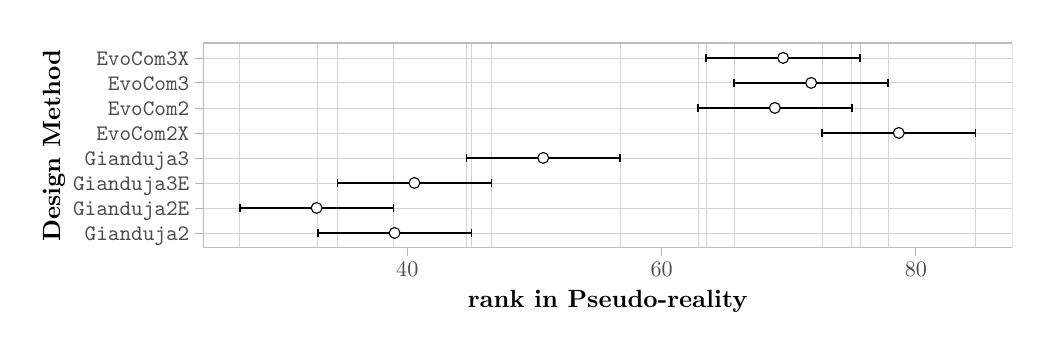
\begin{tikzpicture}[x=1pt,y=1pt]
\definecolor{fillColor}{RGB}{255,255,255}
\path[use as bounding box,fill=fillColor,fill opacity=0.00] (0,0) rectangle (361.35,108.41);
\begin{scope}
\path[clip] (  0.00,  0.00) rectangle (361.35,108.40);
\definecolor{drawColor}{RGB}{255,255,255}
\definecolor{fillColor}{RGB}{255,255,255}

\path[draw=drawColor,line width= 0.6pt,line join=round,line cap=round,fill=fillColor] (  0.00,  0.00) rectangle (361.35,108.40);
\end{scope}
\begin{scope}
\path[clip] ( 63.34, 28.81) rectangle (355.85,102.90);
\definecolor{fillColor}{RGB}{255,255,255}

\path[fill=fillColor] ( 63.34, 28.81) rectangle (355.85,102.90);
\definecolor{drawColor}{RGB}{211,211,211}

\path[draw=drawColor,line width= 0.3pt,line join=round] ( 63.34, 79.41) --
	(355.85, 79.41);

\path[draw=drawColor,line width= 0.3pt,line join=round] ( 63.34, 88.45) --
	(355.85, 88.45);

\path[draw=drawColor,line width= 0.3pt,line join=round] ( 63.34, 34.23) --
	(355.85, 34.23);

\path[draw=drawColor,line width= 0.3pt,line join=round] ( 63.34, 43.27) --
	(355.85, 43.27);

\path[draw=drawColor,line width= 0.3pt,line join=round] ( 63.34, 61.34) --
	(355.85, 61.34);

\path[draw=drawColor,line width= 0.3pt,line join=round] ( 63.34, 52.30) --
	(355.85, 52.30);

\path[draw=drawColor,line width= 0.3pt,line join=round] ( 63.34, 97.48) --
	(355.85, 97.48);

\path[draw=drawColor,line width= 0.3pt,line join=round] ( 63.34, 70.37) --
	(355.85, 70.37);

\path[draw=drawColor,line width= 0.2pt,line join=round] (297.76, 28.81) -- (297.76,102.90);

\path[draw=drawColor,line width= 0.2pt,line join=round] (342.55, 28.81) -- (342.55,102.90);

\path[draw=drawColor,line width= 0.2pt,line join=round] (310.89, 28.81) -- (310.89,102.90);

\path[draw=drawColor,line width= 0.2pt,line join=round] (300.77, 28.81) -- (300.77,102.90);

\path[draw=drawColor,line width= 0.2pt,line join=round] (132.20, 28.81) -- (132.20,102.90);

\path[draw=drawColor,line width= 0.2pt,line join=round] (160.37, 28.81) -- (160.37,102.90);

\path[draw=drawColor,line width= 0.2pt,line join=round] (167.54, 28.81) -- (167.54,102.90);

\path[draw=drawColor,line width= 0.2pt,line join=round] (214.08, 28.81) -- (214.08,102.90);

\path[draw=drawColor,line width= 0.2pt,line join=round] (242.20, 28.81) -- (242.20,102.90);

\path[draw=drawColor,line width= 0.2pt,line join=round] (286.99, 28.81) -- (286.99,102.90);

\path[draw=drawColor,line width= 0.2pt,line join=round] (255.32, 28.81) -- (255.32,102.90);

\path[draw=drawColor,line width= 0.2pt,line join=round] (245.21, 28.81) -- (245.21,102.90);

\path[draw=drawColor,line width= 0.2pt,line join=round] ( 76.64, 28.81) -- ( 76.64,102.90);

\path[draw=drawColor,line width= 0.2pt,line join=round] (104.81, 28.81) -- (104.81,102.90);

\path[draw=drawColor,line width= 0.2pt,line join=round] (111.97, 28.81) -- (111.97,102.90);

\path[draw=drawColor,line width= 0.2pt,line join=round] (158.52, 28.81) -- (158.52,102.90);
\definecolor{drawColor}{RGB}{0,0,0}

\path[draw=drawColor,line width= 0.6pt,line join=round] (297.76, 78.06) --
	(297.76, 80.77);

\path[draw=drawColor,line width= 0.6pt,line join=round] (297.76, 79.41) --
	(242.20, 79.41);

\path[draw=drawColor,line width= 0.6pt,line join=round] (242.20, 78.06) --
	(242.20, 80.77);

\path[draw=drawColor,line width= 0.6pt,line join=round] (342.55, 69.02) --
	(342.55, 71.73);

\path[draw=drawColor,line width= 0.6pt,line join=round] (342.55, 70.37) --
	(286.99, 70.37);

\path[draw=drawColor,line width= 0.6pt,line join=round] (286.99, 69.02) --
	(286.99, 71.73);

\path[draw=drawColor,line width= 0.6pt,line join=round] (310.89, 87.09) --
	(310.89, 89.80);

\path[draw=drawColor,line width= 0.6pt,line join=round] (310.89, 88.45) --
	(255.32, 88.45);

\path[draw=drawColor,line width= 0.6pt,line join=round] (255.32, 87.09) --
	(255.32, 89.80);

\path[draw=drawColor,line width= 0.6pt,line join=round] (300.77, 96.13) --
	(300.77, 98.84);

\path[draw=drawColor,line width= 0.6pt,line join=round] (300.77, 97.48) --
	(245.21, 97.48);

\path[draw=drawColor,line width= 0.6pt,line join=round] (245.21, 96.13) --
	(245.21, 98.84);

\path[draw=drawColor,line width= 0.6pt,line join=round] (132.20, 41.91) --
	(132.20, 44.62);

\path[draw=drawColor,line width= 0.6pt,line join=round] (132.20, 43.27) --
	( 76.64, 43.27);

\path[draw=drawColor,line width= 0.6pt,line join=round] ( 76.64, 41.91) --
	( 76.64, 44.62);

\path[draw=drawColor,line width= 0.6pt,line join=round] (160.37, 32.87) --
	(160.37, 35.59);

\path[draw=drawColor,line width= 0.6pt,line join=round] (160.37, 34.23) --
	(104.81, 34.23);

\path[draw=drawColor,line width= 0.6pt,line join=round] (104.81, 32.87) --
	(104.81, 35.59);

\path[draw=drawColor,line width= 0.6pt,line join=round] (167.54, 50.95) --
	(167.54, 53.66);

\path[draw=drawColor,line width= 0.6pt,line join=round] (167.54, 52.30) --
	(111.97, 52.30);

\path[draw=drawColor,line width= 0.6pt,line join=round] (111.97, 50.95) --
	(111.97, 53.66);

\path[draw=drawColor,line width= 0.6pt,line join=round] (214.08, 59.98) --
	(214.08, 62.69);

\path[draw=drawColor,line width= 0.6pt,line join=round] (214.08, 61.34) --
	(158.52, 61.34);

\path[draw=drawColor,line width= 0.6pt,line join=round] (158.52, 59.98) --
	(158.52, 62.69);

\path[draw=drawColor,line width= 0.4pt,line join=round,line cap=round,fill=fillColor] (269.98, 79.41) circle (  1.96);

\path[draw=drawColor,line width= 0.4pt,line join=round,line cap=round,fill=fillColor] (314.77, 70.37) circle (  1.96);

\path[draw=drawColor,line width= 0.4pt,line join=round,line cap=round,fill=fillColor] (283.11, 88.45) circle (  1.96);

\path[draw=drawColor,line width= 0.4pt,line join=round,line cap=round,fill=fillColor] (272.99, 97.48) circle (  1.96);

\path[draw=drawColor,line width= 0.4pt,line join=round,line cap=round,fill=fillColor] (104.42, 43.27) circle (  1.96);

\path[draw=drawColor,line width= 0.4pt,line join=round,line cap=round,fill=fillColor] (132.59, 34.23) circle (  1.96);

\path[draw=drawColor,line width= 0.4pt,line join=round,line cap=round,fill=fillColor] (139.75, 52.30) circle (  1.96);

\path[draw=drawColor,line width= 0.4pt,line join=round,line cap=round,fill=fillColor] (186.30, 61.34) circle (  1.96);
\definecolor{drawColor}{RGB}{190,190,190}

\path[draw=drawColor,line width= 0.6pt,line join=round,line cap=round] ( 63.34, 28.81) rectangle (355.85,102.90);
\end{scope}
\begin{scope}
\path[clip] (  0.00,  0.00) rectangle (361.35,108.41);
\definecolor{drawColor}{gray}{0.30}

\node[text=drawColor,anchor=base east,inner sep=0pt, outer sep=0pt, scale=  0.80] at ( 58.39, 76.66) {\texttt{EvoCom2}};

\node[text=drawColor,anchor=base east,inner sep=0pt, outer sep=0pt, scale=  0.80] at ( 58.39, 85.69) {\texttt{EvoCom3}};

\node[text=drawColor,anchor=base east,inner sep=0pt, outer sep=0pt, scale=  0.80] at ( 58.39, 31.48) {\texttt{Gianduja2}};

\node[text=drawColor,anchor=base east,inner sep=0pt, outer sep=0pt, scale=  0.80] at ( 58.39, 40.51) {\texttt{Gianduja2E}};

\node[text=drawColor,anchor=base east,inner sep=0pt, outer sep=0pt, scale=  0.80] at ( 58.39, 58.58) {\texttt{Gianduja3}};

\node[text=drawColor,anchor=base east,inner sep=0pt, outer sep=0pt, scale=  0.80] at ( 58.39, 49.55) {\texttt{Gianduja3E}};

\node[text=drawColor,anchor=base east,inner sep=0pt, outer sep=0pt, scale=  0.80] at ( 58.39, 94.73) {\texttt{EvoCom3X}};

\node[text=drawColor,anchor=base east,inner sep=0pt, outer sep=0pt, scale=  0.80] at ( 58.39, 67.62) {\texttt{EvoCom2X}};
\end{scope}
\begin{scope}
\path[clip] (  0.00,  0.00) rectangle (361.35,108.41);
\definecolor{drawColor}{gray}{0.70}

\path[draw=drawColor,line width= 0.3pt,line join=round] ( 60.59, 79.41) --
	( 63.34, 79.41);

\path[draw=drawColor,line width= 0.3pt,line join=round] ( 60.59, 88.45) --
	( 63.34, 88.45);

\path[draw=drawColor,line width= 0.3pt,line join=round] ( 60.59, 34.23) --
	( 63.34, 34.23);

\path[draw=drawColor,line width= 0.3pt,line join=round] ( 60.59, 43.27) --
	( 63.34, 43.27);

\path[draw=drawColor,line width= 0.3pt,line join=round] ( 60.59, 61.34) --
	( 63.34, 61.34);

\path[draw=drawColor,line width= 0.3pt,line join=round] ( 60.59, 52.30) --
	( 63.34, 52.30);

\path[draw=drawColor,line width= 0.3pt,line join=round] ( 60.59, 97.48) --
	( 63.34, 97.48);

\path[draw=drawColor,line width= 0.3pt,line join=round] ( 60.59, 70.37) --
	( 63.34, 70.37);
\end{scope}
\begin{scope}
\path[clip] (  0.00,  0.00) rectangle (361.35,108.41);
\definecolor{drawColor}{gray}{0.70}

\path[draw=drawColor,line width= 0.3pt,line join=round] (137.18, 26.06) --
	(137.18, 28.81);

\path[draw=drawColor,line width= 0.3pt,line join=round] (229.07, 26.06) --
	(229.07, 28.81);

\path[draw=drawColor,line width= 0.3pt,line join=round] (320.95, 26.06) --
	(320.95, 28.81);
\end{scope}
\begin{scope}
\path[clip] (  0.00,  0.00) rectangle (361.35,108.41);
\definecolor{drawColor}{gray}{0.30}

\node[text=drawColor,anchor=base,inner sep=0pt, outer sep=0pt, scale=  0.80] at (137.18, 18.35) {40};

\node[text=drawColor,anchor=base,inner sep=0pt, outer sep=0pt, scale=  0.80] at (229.07, 18.35) {60};

\node[text=drawColor,anchor=base,inner sep=0pt, outer sep=0pt, scale=  0.80] at (320.95, 18.35) {80};
\end{scope}
\begin{scope}
\path[clip] (  0.00,  0.00) rectangle (361.35,108.41);
\definecolor{drawColor}{RGB}{0,0,0}

\node[text=drawColor,anchor=base,inner sep=0pt, outer sep=0pt, scale=  0.90] at (209.60,  7.44) {\bfseries rank in Pseudo-reality};
\end{scope}
\begin{scope}
\path[clip] (  0.00,  0.00) rectangle (361.35,108.41);
\definecolor{drawColor}{RGB}{0,0,0}

\node[text=drawColor,rotate= 90.00,anchor=base,inner sep=0pt, outer sep=0pt, scale=  0.90] at ( 11.71, 65.86) {\bfseries Design Method};
\end{scope}
\end{tikzpicture}

\caption{
Thick gray boxes represent the results of robot experiments;
Thick white boxes those of pseudo-reality; thin gray ones,
those of simulations.}
\label{fig:task1res}
\end{figure}


\end{document}
